
We first examine human verb selection in a constrained setting to better
understand what performance we should demand of computational approaches.  While
we know that humans make incremental predictions across sentences, we do not
know how skilled they are in doing so. While it's possible that machines---with
unbounded memory and access to Internet-sized data---could do better than
humans, this study allows us to appropriately gauge our expectations for
computational systems.

We use crowdsourcing to measure how well novice humans can predict the final
verb phrase of incomplete Japanese sentences in a multiple choice setting.  We
use Japanese text of the Kyoto Free Translation Task
corpus~\cite[\abr{kft}]{neubig2011kyoto}, a collection of Wikipedia articles in
English and Japanese, representing standard, grammatical text and readily usable
for future \abr{sov}-\abr{svo} machine translation experiments.

\subsection{Extracting Verbs and Sentences}
\label{sec:human_prediction}

This section describes the data sources, preparation, and methodology
for crowdsourced verb prediction.  Given an incomplete sentence,
participants select a sentence-final verb phrase containing a verb
from a list of four choices to complete the sentence, one of which is
the original completion.

We randomly select 200 sentences from the development set of the
\abr{kft} corpus~\cite{neubig2011kyoto}.  We use these data because the
sentences are from Wikipedia articles and thus represent widely-read,
grammatical sentences.  These data are directly comparable to our computational
experiments and readily usable for future \abr{sov}-\abr{svo} machine translation
experiments.

We ask participants to predict a ``verb chunk'' that would be natural
for humans.  More technically, this is a
sentence-final \emph{bunsetsu}.\footnote{{A \it bunsetsu} is a commonly
used linguistic unit in Japanese, roughly equivalent to an English
phrase: a collection of content words and zero or more functional
words. Japanese verb \textit{bunsetsu} often encompass complex
conjugation. For example, a verb phrase 読みたくなかった
(read-\abr{desi-neg-past}), meaning `didn't want to read', has
multiple tokens capturing tense, negation, etc.\ necessary for
translation.}  We identify verb \textit{bunsetsu} with a dependency
parser~\cite{kurohashi1994kn}.  Of interest are \textit{bunsetsu} at
the end of a sentence that contain a verb.  We also use
\textit{bunsetsu} for segmenting the incomplete sentences we show to
humans, only segmenting between \textit{bunsetsu} to ensure each
segment is a meaningful unit.

\paragraph{Answer Choice Selection}

We display the correct verb \textit{bunsetsu} and three incorrect
\textit{bunsetsu} completions as choices that occur in the data with
frequency close to the correct answer in the overall corpus. We
manually inspect the incorrect answers to ensure that these choices
are semantically distant, i.e., excluding synonyms or troponyms.

\paragraph{Sentence Presentation}

We create two test sets of truncated sentences from the \abr{kft}
corpus: The first, the {\bf full context set},
includes all but the final \textit{bunsetsu}---i.e., the verb
phrase---to guess.  The second set, the {\bf random length set},
contains the same sentences truncated at predetermined, random
\textit{bunsetsu} boundaries.  The average sentence length is nine
\textit{bunsetsu}, with a maximum of fourteen and minimum of three. We
display sentences in the original Japanese script.

Participants view the task as a game of guessing the final verb.  Each
fragment has four concurrently displayed completion options, as in
the prompt (2) and answers (3). Users receive no feedback from
the interface.





















We use CrowdFlower\footnote{http://www.crowdflower.com/} to collect
participants' answers, at a total cost of approximately \abr{usd}\$300. From
an initial pool of fifty-six participants, we remove twenty via a
Japanese fluency screening. We verify the efficacy of this test with
non-native but highly proficient Japanese learners; none passed. We
collect five judgments per sentence from each participant.

\begin{enumerate}[(2)]
\listsep
\item \label{sent-ex}
       \gl{谷崎潤一郎は}{Junichiro Tanizaki-\abr{top}}
       \gl{数寄屋を}{tea-ceremony house-\abr{obj}}

\end{enumerate}
\begin{enumerate}[(3)]
\listsep
\item \label{sent-ex-choices}
\begin{enumerate*}
  \item \gl{好んだ}{like-PAST}
  \item \gl{変えられた}{change-PASS CAP-PAST}
  \item \gl{始まったとされている}{begin-PAST-COMP-suppose-AUX.PRES}
  \item \gl{増やしていた}{increase-AUX.PAST}
\end{enumerate*}
\end{enumerate}




\subsection{Presenting Partial and Complete Sentences}


The first task, on the {\bf full context set}, shows how humans
predict the sentence-final verb chunk with all context available.  The
second task, on the {\bf random length set}, shows how the amount of
revealed data affects the predictability of the final verb chunk. We
examine a correlation between the length of the pre-verb sentence
fragment and participants' accuracy (Figure~\ref{fig:full_prefix}).




  Psycholinguistic experiments using lexical decision tasks suggest Japanese
  speakers start syntactic processing by using case---the type and number of
  case-marked arguments---before the verb's availability~\cite{yamashita2000}.
  We also examine the correlation between the number of case markers\footnote{In
    this study, we counted case markers that mark nominative ({\it -ga}),
    accusative ({\it -wo}), ablative ({\it -kara}), and dative ({\it -ni}).}
  and accuracy.  It is likely that the number of case markers and the length of
  the sentence fragment are confounded; so, we create a measure, the proportion
  of case markers to the overall sentence information (the number of case
  markers in the fragment divided by the number of {\it bunsetsu} chunks). We
  call this \textbf{case density}.


\subsection{Results of Human Experiments}
\label{sec:results}


In the {\bf full context set}, average accuracy over 200 sentences is 81.1\%,
significantly better than chance $(p<2.2 \cdot 10^{-16})$.
Figure~\ref{fig:full_prefix} shows the accuracy per sentence length as defined
by the {\it bunsetsu} unit.  A one-way \abr{anova} reveals a significant effect
of the sentence length $(F(1,998)=7.512, p<0.00624)$, but not the case density
$(F(1,998)=1.2, p=0.274)$.

\begin{figure}[t!]
 \begin{center}
 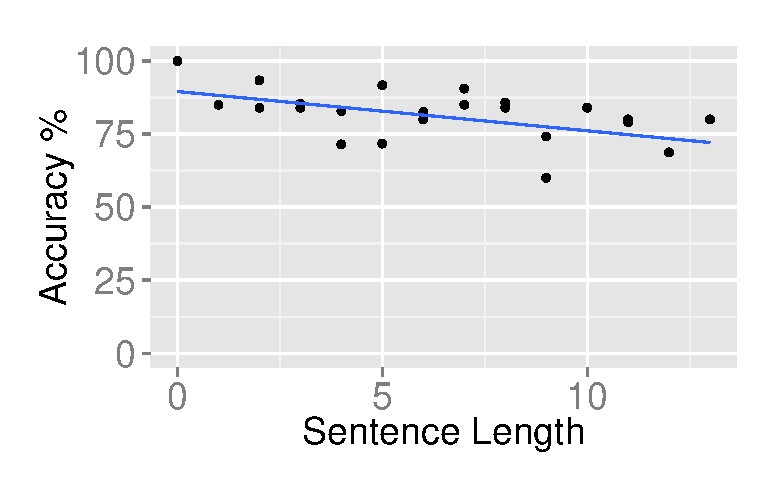
\includegraphics[width=1.0\linewidth]{2016_conll_verbpred/figures/full-pref-len}
 \caption{Full context set: Accuracy is generally high, but
   slightly decreases on longer, more complicated sentences, averaging
   81.1\%.}
 \label{fig:full_prefix}
  \end{center}
\end{figure}

In the {\bf random length set}, average accuracy over 200 sentences is 54.2\%,
significantly better than chance $(t(199) = 11.8205,
p<2.2\cdot10^{-16})$. Figure~\ref{fig:rand_prefix} shows the accuracy per
percentage of length of the presented sentence fragment.  A one-way \abr{anova}
reveals a significant effect of the sentence length
$(F(1,998)=57.44, p<7.94\cdot10^{-14})$.  We also find a significant effect of
the case density $(F(1,998)=5.884, p=0.0155)$.













\begin{figure}[t!]
 \begin{center}
 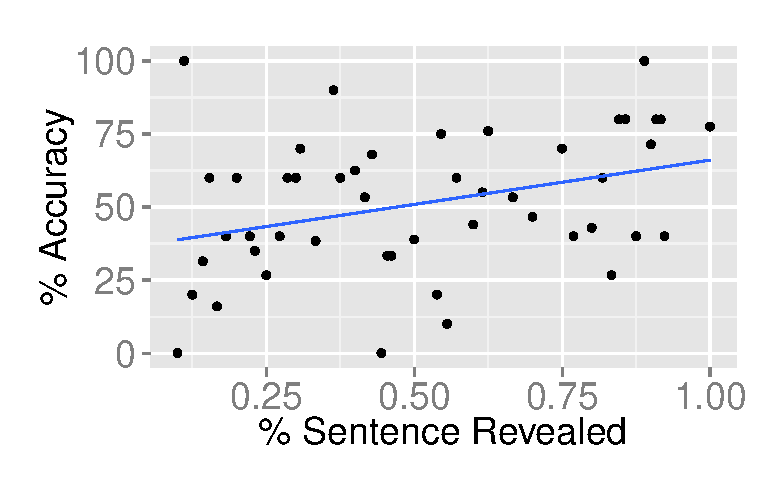
\includegraphics[width=1.0\linewidth]{2016_conll_verbpred/figures/rand-pref-len}
 \caption{Random length set: The accuracy of human verb predictions
   reliably increases as more of the sentence is revealed. }
 \label{fig:rand_prefix}
\end{center}
\end{figure}

\subsection{Discussion}

Predictability increases with the percent of the sentence available in all of
our experiments.  By the end of the sentence, the verb chunks are highly
predictable by humans in the multiple choice setting.  Participants choose the
final verb more accurately as they gain access to more case markers in the {\bf
  random length set} but not in the {\bf full context set}.

Case density is a significant factor in predictive accuracy on the
{\bf random length set} for humans, suggesting that case is more
helpful in predicting a sentence-final verb when the preceding
contextual information is insufficient. The following example
illustrates how case helps in prediction. The nominative and
accusative markers greatly narrow the choices, as shown in
(4).\footnote{A recent psycholinguistics study on incremental Japanese
  verb-final processing~\cite{momma2015timing} argues that native
  Japanese speakers plan verbs in advance, before the articulation of
  object nouns, but not subject nouns. Since case markers assign the
  roles of subject and object in Japanese, we expect that a high ratio
  of case markers to words will increase predictability of verbs. In
  addition, \newcite{yamashita1997effects} argues that the
  \textit{variety} of case markers increases predictability just
  before the verb.} Our results further support the proposition case
markers modulate predictability in \abr{sov} verb-final processing.
















































\begin{enumerate}[(4)]
 \setlength{\parskip}{-0.1cm}
 \item \label{quat-ex2}
  \gl{江戸幕府区-{\bf が}}{Edo shogunate-{\bf\abr{nom}}}
  \gl{成立すると}{establish-do-{\bf\abr{conj}}}
  \gl{寺院法度-{\bf に}-より}{temple-prohibition-etc.-\abr{acc}-for}
  \gl{---}{} \\
  `After Edo shogunate has established, due to the temple prohibition etc. ---'
\end{enumerate}






















In other cases, there exist choices, which, while incorrect, could naturally
complete the sentence.  These questions are frequently missed. For instance, in
one 90\% revealed sentence, the participant has the choices: (i) 収め
る (put-\abr{pres}), (ii) 厳しくなる (strict-become), (iii) {\it 収録されている}
(record-do.\abr{pass-aux.pres}), and (iv) 務める (work-\abr{pres}).  Choice (i)
is the correct answer, but choice (iii) is a reasonable choice for a Japanese
speaker.  All participants missed this question, and all chose the same wrong
answer (iii).  We leave a cloze task where participants can freely fill in the
sentence-final to future work.

These results provide a basis of comparison for automatic prediction.  In the
next section, we examine whether computational models can predict final
verbs and compare the models' performance to that of humans.